\setcounter{section}{4}
\setcounter{subsection}{1}
\setcounter{question}{0}
\setcounter{hint}{0} % Only for first assignment in chapter

%%%%%%%%%%%%%%%%%%%%%%%%%%%%%%%%%%%%%%%%%%%%%%%%%%%%%%%%%%%%%%%%%%%%%%%%%%%
% Assignment 4.1: Calculating covariance and correlation by hand
%%%%%%%%%%%%%%%%%%%%%%%%%%%%%%%%%%%%%%%%%%%%%%%%%%%%%%%%%%%%%%%%%%%%%%%%%%%

\handassignment{Calculating covariance and correlation by hand}

The manager of a local branch of a supermarket chain in the Netherlands has had a bad year last year and wants to improve their sales. Her co-worker has brought up the idea to spend more money on advertising in the neighborhoods that are further away from the store. The co-worker thinks that customers that live further away might visit the supermarket less frequently. He believes that making an effort to attract these people may prove to be profitable for the store. Realizing that her branch currently does not spend a notable amount of money on advertising at all, the manager is interested to know about the \concept{relationship} between the distance a customer lives from the store and the average number of times they visit the store per week. \\

The manager requests her co-worker to ask the customers at his counter some questions when they check out at his counter. He is instructed to ask them a) how many times, on average, they visit the store per week and b) the number of kilometers they live from the store. The co-worker asks eight customers and reports the findings to his manager. \\

\question{
    What kind of \concept{relationship} do you expect to see? Formulate your answer in terms of the direction of the \concept{relationship}.
}

\twolineanswerbox

The manager sits down with her co-worker, writes down the numbers, and creates a scatter plot of the data. She displays the distance a customer lives from the store (in kilometers) on the \textit{x-axis} and their average number of visits per week on the \textit{y-axis}. 

\clearpage % Page break

\begin{minipage}[t]{0.4\textwidth}
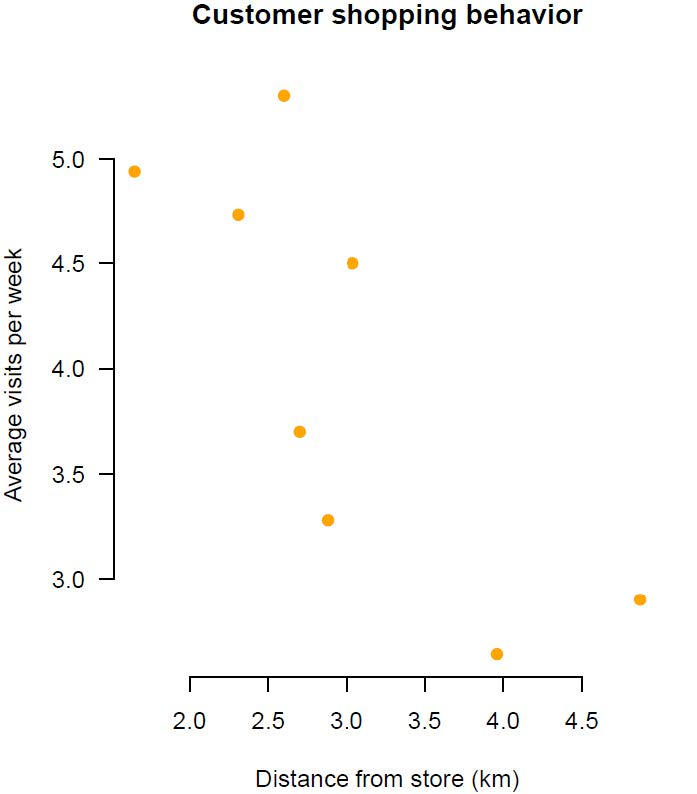
\includegraphics[width=\textwidth]{Files/Images/covariance.jpg}
\end{minipage}%
\begin{minipage}[t]{0.6\textwidth}
\vspace*{-7cm}
\begin{center}
    \begin{tabular}{|c|c|c|c|c|c|}
    \hline 
    $i$ & $x_i$ & $y_i$ & $(x_i - \bar{x})$ & $(y_i - \bar{y})$ & $(x_i - \bar{x})(y_i - \bar{y})$ \tstrut\bstrut\\
    \hline
    1 & 4.87 & 2.90 & & &  \tstrut\bstrut\\
    \hline
    2 & 3.04 & 4.50 & & &  \tstrut\bstrut\\
    \hline
    3 & 1.65 & 4.94 & & &  \tstrut\bstrut\\
    \hline
    4 & 2.88 & 3.28 & & &  \tstrut\bstrut\\
    \hline
    5 & 2.31 & 4.73 & & &  \tstrut\bstrut\\
    \hline
    6 & 3.96 & 2.64 & & &  \tstrut\bstrut\\
    \hline
    7 & 2.70 & 3.70 & & &  \tstrut\bstrut\\
    \hline
    8 & 2.60 & 5.30 & & &  \tstrut\bstrut\\
    \hline
    \end{tabular}
    \end{center}
    
    \hspace*{.5cm} $\bar{x} = $  ............. \hspace*{1cm} $\sum (x_i - \bar{x})(y_i - \bar{y}) = $  ............. \\
    \\
    \hspace*{.5cm} $\bar{y} = $ ............. \hspace*{3.1cm} $n - 1 = $  ............. \\
    \\
    \hspace*{6.5cm} $s_{xy} = $  ............ \\
\end{minipage}%

\question{
    Use the table above to calculate and fill in the \concept{covariance} $s_{xy}$ between the customer’s distance from the store and their average number of visits per week. 
}

\hint{You can find the complete formula for the \concept{covariance} in the formula sheet.}

\question{
    Interpret the \concept{covariance} from these data. What can you say about the \concept{relationship} between the distance from the store and the average number of visits per week on the basis of this measure?
}

\threelineanswerbox

The \concept{covariance} $s_{xy}$ is a useful measure to get an idea about the extent to which two \concept{variables} change together, but it also has some disadvantages when using it as a measure of the strength of a \concept{relationship}. 

\clearpage % Page break

\question{
    Explain the disadvantage of using the \concept{covariance} $s_{xy}$ as a measure for the strength of this \concept{relationship}. Consider in your answer what would have happened if the co-worker asked the customers how many meters they lived from the store.
}

\threelineanswerbox

To reliably measure the strength of the \concept{relationship}, the manager wants to \concept{standardize} the \concept{covariance} $s_{xy}$ to find out the \concept{correlation} coefficient $r_{xy}$. To do this, she first needs to calculate the sample \concept{standard deviation} of the distance from the store in kilometers ($s_x$) and the sample \concept{standard deviation} of the average number of visits per week($s_y$). \\

\question{
    Calculate $s_x$ and $s_y$ for the data that the co-worker collected. 
}

\hint{You can find the formula for the \concept{standard deviation} in the formula sheet.}

\emptyanswerbox{
    $s_x$: \shortanswerline \hspace*{3cm} $s_y$: \shortanswerline
}

\question{
    Use the sample \concept{standard deviations} and the sample \concept{covariance} to calculate the sample \concept{correlation} $r_{xy}$.
}

\hint{You can find the formula for the \concept{correlation coefficient} $r_{xy}$ in the formula sheet.}

\emptyanswerbox{
    $r_{xy}$: \shortanswerline
}

\question{
   Interpret the \concept{correlation coefficient}. Is this a strong \concept{relationship}?
}

\onelineanswerbox

\clearpage % Page break